\section{Auswertung}
\label{sec:Auswertung}

\subsection{Vorbereitung: Berechnung der Theorie-Werte}

    Es werden die drei Elemente Neodymium, Gadolinium und Dysprosium untersucht, von denen jeweils zwei als dreifach positiv geladene 
    Ione mit drei zweifach negativ geladenen Sauerstoff-Ionen ein Molekül bilden. 
    Ebenfalls haben alle drei Elemente zwei 6s-Elektronen und eine bis zur 5p-Schale. Nur hinsichtlich der Anzahl \# der 4f-Elektronen unterscheiden sie sich. 
    Dies ist auch der Fall, wenn sie im ionisierten Zustand sind: 
    Jeweils zwei 6s-Elektronen und ein 4f-Elektron verschwindet; die Elektronen bis zur 5p-Schale bleiben unverändert. 
    Zur besseren Übersicht werden die Zwischenergebnisse in Tabelle \ref{tab:Theo1} zusammengefasst. 

    Auf der 4f-Schale können sich maximal 14 Elektronen befinden: 
    Die Bahndrehimpulsquantenzahl $l$ kann Werte zwischen $-3$ und $3$ annnehmen, also sieben verschiedene Werte sind möglich. 
    Zusätzlich gibt es für jede Quantenzahl $l$ maximal ein Elektron mit Spin Up und eins mit Spin Down. Daraus resultiert eine maximale Anzahl von vierzehn Elektronen auf dieser Schale. 
    Dementsprechend wird gemäß den Hund'schen Regeln \ref{sub:wauwau} bei einer Elektronenzahl von inklusive sieben 
    die Quantenzahl des Gesamtdrehimpuls durch Addition $L+S$ berechnet, bei einer geringeren Zahl durch Subtraktion $L-S$. 

    Mithilfe der Quantenzahlen wird der Landé-Faktor gemäß Gleichung \eqref{eqn:lande} berechnet. 

    \begin{table}
        \centering
        \caption{Bestimmung der Quantenzahlen.}
        \label{tab:Theo1}
        \begin{tabular}{l c c c c c c}
            \toprule
             & 
            neutral & 
            \multicolumn{4}{c}{ionisiert} \\
            \cmidrule(lr){2-2} \cmidrule(lr){3-7}
            Element &
            \# 4f & 
            \# 4f &
            $S$ & 
            $L$ & 
            $J$ &
            $g_J$ \\
            \midrule
            Nd &  4 & 3 & $3\cdot\sfrac{1}{2}=\sfrac{3}{2}$                       & 6 & $\sfrac{9}{2}$  & 0.727 \\
            Gd &  8 & 7 & $7\cdot\sfrac{1}{2}=\sfrac{7}{2}$                       & 0 & $\sfrac{-7}{2}$ & 2.400 \\
            Dy & 10 & 9 & $7\cdot\sfrac{1}{2}+2\cdot\sfrac{-1}{2}=\frac{5}{2}$    & 5 & $\sfrac{15}{2}$ & 1.333 \\
            \bottomrule
        \end{tabular}
    \end{table}

    Zur Berechnung des theoretisch zu erwartenden Werts der Suszeptibilität $\chi$ wird ebenfalls die Anzahl $N$ der atomaren magnetischen 
    Dipolmomente pro Volumeneinheit benötigt. 
    Hierfür wird die molare Masse zu 
    \begin{equation*}
        M_\text{Molekül}=3M_\text{O}+2M_\text{SE}
    \end{equation*}
    bestimmt mit der molaren Masse des Sauerstoff und der des jeweiligen Seltenen-Erd-Metalls. 
    Je Molekül gibt es also zwei magnetische atomare Dipolmomente, die durch die Ionen des Metalls verursacht werden und 
    deren Größe in Tabelle \ref{tab:Theo1} bestimmt werden.

    Die Stoffmenge der vorliegenden Proben ist 
    \begin{equation*}
        n_\text{Molekül}=\frac{m}{M_\text{Molekül}}
    \end{equation*}
    mit der Masse $m$. 
    Sie gibt die Anzahl der Teilchen in Mol an, die in der Probe enthalten sind. 
    Dementsprechend berechnet sich die Anzahl der Moleküle pro Volumen durch Division der Stoffmenge mit dem Volumen. 
    Zu beachten ist hierbei, dass erneut ein effektives Volumen und somit auch die effektive Querschnittsfläche \eqref{eqn:effQ} verwendet 
    werden muss, da es sich um ein dekomprimiertes Pulver und nicht um einen Ein-Kristall handelt.
    Multipliziert man dies mit zwei, ergibt sich die Anzahl der Mole der positiv geladenen Seltenen-Erd-Ionen in der gegebenen Probe:
    \begin{equation*}
        N_\text{Ione,mol}=2\cdot\frac{n_\text{Molekül}}{V_\text{Probe,eff}}=2\cdot\frac{n_\text{Molekül}}{Q_\text{eff}L}
        =2\cdot\frac{\rho _\text{w} n_\text{Molekül}}{m}\,.
    \end{equation*}
    Die Dichte $\rho _\text{w}$ steht im Experiment bereits zur Verfügung und muss nicht extra aufgenommen werden. 
    Die Anzahl $N$ der Teilchen ohne Einheiten pro Volumeneinheit wird durch Multiplikation der Avogadro-Konstante $\symup{N}_\text{A}$ erreicht.
    \begin{equation*}
        N=N_\text{Ione,mol}\cdot \symup{N}_\text{A}=\frac{2\symup{N}_\text{A}\rho_\text{w}}{M_\text{Molekül}}
    \end{equation*}
    Die entsprechenden Daten dazu sind in Tabelle \ref{tab:Theo2} dargestellt. 
    Die Werte für die molare Masse sind \cite[610]{kohlrausch} entnommen.
    Die des Sauerstoffs ist $M_\text{O}=\SI{15.9994}{\gram\per\mole}$.

    \begin{table}
        \centering
        \caption{}
        \label{tab:Theo2}
        \begin{tabular}{l c c S[table-format=2.2] S[table-format=1.2] c}
            \toprule
            Element & 
            $M_\text{SE}\,/\,\si{\gram\per\mole}$ &
            $M_\text{Mol}\,/\,\si{\gram\per\mole}$ &
            $m\,/\,\si{\gram}$ & 
            $\rho_\text{w}\,/\,\si{\gram\per\cubic\centi\meter}$ &
            $N\,/\,\SI{e28}{\per\cubic\meter}$ \\
            \midrule
            Nd & 144.22 & 336.44 & 9.0   & 7.24 & 2.592 \\
            Gd & 157.25 & 362.50 & 14.08 & 7.40 & 2.459 \\
            Dy & 162.50 & 373.00 & 14.38 & 7.8  & 2.519 \\
            \bottomrule
        \end{tabular}
    \end{table}

    Gemäß Gleichung \eqref{eqn:chii} ist die Suszeptibilität temperaturabhängig. 
    Der Versuch ist bei Raumtemperatur und Sommerwetter durchgeführt worden. 
    Die Temperatur wird deshalb mit ${T\approx(\num{273.15}+\num{23.85})\si{\kelvin}=\SI{297}{\kelvin}}$ abgeschätzt.
    Daraus ergeben sich für die Suszeptibilität folgende theoretische Werte:
    \begin{equation}
        \chi _\text{Nd}=\num{2.98e-03} 
        \label{eqn:chi1}
    \end{equation}
    \begin{equation}
        \chi _\text{Gd}=\num{10.9e-03} 
    \end{equation}
    \begin{equation}
        \chi _\text{Dy}=\num{25.1e-03} 
        \label{eqn:chi3}
    \end{equation}
        
        


\subsection{Filterkurve des Selektivverstärkers}

    \begin{figure}
        \centering
        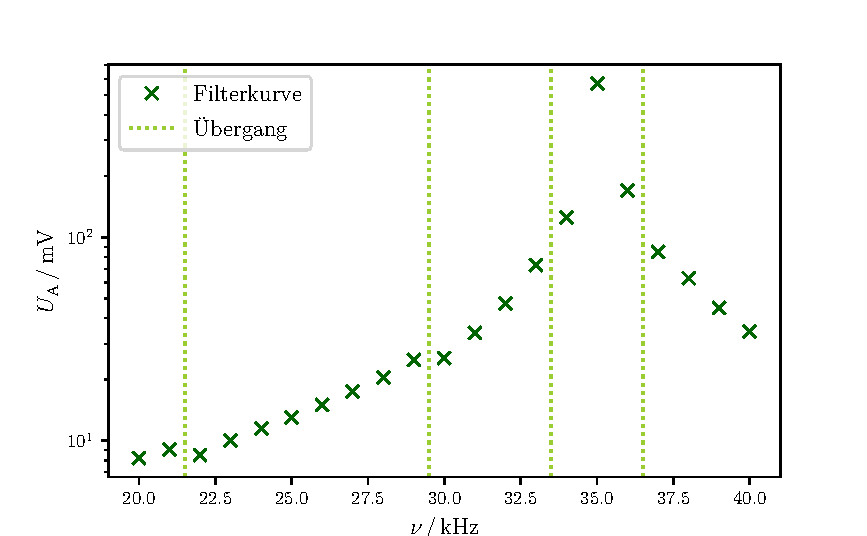
\includegraphics[width=0.75\textwidth]{plots/Filterkurve.pdf}
        \caption{Filterkurve des Selektivverstärkers zur Bestimmung der Durchlassfrequenz.}
        \label{fig:Filterkurve}
    \end{figure}

    Die Messwerte sind in Abbildung \ref{fig:Filterkurve} dargestellt, das bedeutet, dass die Ausgangsspannung gegen die Frequenz aufgetragen ist. 
    Wichtig ist hierbei das Maximum, das sich eindeutig bei $\nu=\SI{35}{\kilo\hertz}$ feststellen lässt. 
    Dementsprechend wird ebendiese Frequenz für die weiteren Messungen benutzt. 
    Ebenfalls ist aus der Graphik ersichtlich, wenn der Messbereich des Voltmeters gewechselt worden ist. 
%    Die Messwerte an den Übergängen können entsprechend leicht variieren. --> in der Diskussion

\subsection{Berechnung der experimentellen Werte für die Suszeptibilität}

    Die Kenngrößen und Messwerte werden der Übersicht halber in den Tabellen \ref{tab:KennGr} und \ref{tab:Messwerte} zusammengefasst.
    Bereits berücksichtigt wird hierbei die Verstärkung der gemessenen Brückenspannung um den Faktor $100$. Entsprechend 
    wird $\SI{1}{\milli\volt}$ der Messwert $\SI{1e-2}{\milli\volt}$ zugeordnet.
    \begin{table}
        \centering
        \caption{Kenngrößen der Messappaturen.}
        \label{tab:KennGr}
        \begin{tabular}{l l}
            \toprule
            Größe & Wert \\
            \midrule
            Frequenz $\nu$                  & $\SI{35.00}{\kilo\hertz}$ \\
            Speisespannung $U_\text{Sp}$    & $\SI{1.0}{\volt}$ \\
            Windungszahl $n$                & $\num{250}$ \\
            Querschnittsfläche Spule $F$          & $\SI{86.6}{\milli\meter\squared}$ \\
            Spulenlänge $l$                 & $\SI{135}{\milli\meter}$ \\
            \bottomrule
        \end{tabular}
    \end{table}
    \begin{table}
        \centering
        \caption{Messwerte der Brückenwiderstände und -spannung in Abhängigkeit der Spulenfüllung.}
        \label{tab:Messwerte}
        \begin{tabular}{l c c c c}
            \toprule
            Füllung & $R_3\,/\,\si{\ohm}$ & $\Delta R\,/\,\si{\ohm}$ & $R_4\,/\,\si{\ohm}$ & $U_\text{Br}\,/\,\SI{e-5}{\volt}$ \\
            \midrule
            ohne    & 2.58 &  -   & 2.42 & 1.50 \\ 
            Nd      & 2.73 & 0.15 & 2.27 & 1.45 \\
            Gd      & 3.47 & 0.74 & 1.53 & 1.35 \\
            Dy      & 4.16 & 1.43 & 0.84 & 1.15 \\
            \bottomrule
        \end{tabular}
    \end{table}
    
    Nun wird auf zwei Wegen die Suszeptibilität berechnet: Einmal $\chi_1$ über Gleichung \eqref{eqn:hatschi} mithilfe der Brückenspannung; 
    und dann noch $\chi_2$ über \eqref{eqn:chii2}, die die Widerstände benutzt. 
    Die Querschnittsfläche $Q$ wird jeweils durch die effektive Querschnittsfläche $Q_\text{eff}$ aus \eqref{eqn:effQ} substituiert. 
    Es ergeben sich die in Tabelle \ref{tab:chii} zusammengefassten Werte. 
    \begin{table}
        \centering
        \caption{Die experimentell berechneten Werte für die Suszeptibilität.}
        \label{tab:chii}
        \begin{tabular}{l c c}
            \toprule
            Element & $\chi_1$ &  $\chi_2$ \\
            \midrule
            Nd & $\num{5.45e-4}$ & 1.03 \\
            Gd & $\num{3.32e-4}$ & 3.15 \\
            Dy & $\num{2.92e-4}$ & 4.82 \\
            \bottomrule
        \end{tabular}
    \end{table}